\section{Descripción del método TAMA}
\label{sec:ant_tama}

\begin{figure}[t!]
\centering
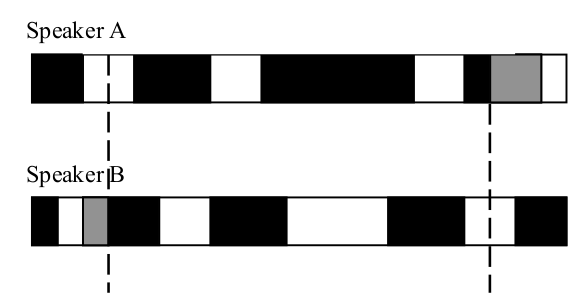
\includegraphics[width=10cm]{images/tama.png}
\caption{Gráfico de la separación del diálogo en ventanas. Fuente \cite{KOU2008}}

\label{tama}
\end{figure}

En \cite{KOU2008} se introdujo un método novedoso para el análisis del \entrainment acústico-prosódico. Esta técnica consiste, a grandes rasgos, en armar dos series de tiempo para cada uno de los interlocutores y luego utilizar herramientas de análisis sobre las series construídas. Una serie de tiempo, en términos coloquiales, es una colección cronológica de observaciones, como pueden ser los valores de las acciones de una empresa a lo largo del tiempo, o la cantidad de lluvia medida en milímetros para cada mes de cierto año. En el Apéndice \ref{sec:time_series} describimos más en detalle los conceptos básicos sobre series de tiempo.

Para construir la serie de tiempo de cada hablante se debe, en primer lugar, dividir el diálogo en ventanas solapadas de igual tamaño. A la diferencia entre ventana y ventana llamaremos \emph{frame step}, y al tamaño de ventana \emph{frame length}. Consideraremos sólo los segmentos de habla que se encuentren dentro de cada ventana; aquellos que atraviesen los límites de las ventanas serán cortados para que se mantengan dentro de éste. En la Figura \ref{tama} se ilustra el proceso: las líneas punteadas marcan los límites de la ventana, los intervalos coloreados en negro los segmentos de habla, y en gris los segmentos cortados.

Como producto de esto, nuestro corpus queda dividido en una sucesión ventanas solapadas. En el trabajo original \cite{KOU2008}, se usa un step de 10 segundos, y un tamaño de ventana de 20 segundos, dando como resultado un solapamiento del 50\%. En la Sección \ref{sec:window_selection}, describimos la elección del tamaño de ventana que hicimos en base al corpus utilizado.


Una vez que la conversación se ha partido en ventanas mediante el proceso descripto, se calculan los valores de la serie de tiempo para cada hablante y cada variable acustico-prosódicas (por ejemplo el pitch) mediante el siguiente cálculo:

\begin{equation}
    \mu = \sum\limits_{i=1}^N f_i d_i^\prime \label{eq:tama_mean}\\
\end{equation}

\noindent donde $i$ itera sobre las elocuciones dentro del \emph{frame}, $d_i^\prime$ es la duración relativa del segmento (respecto del tiempo total hablado en toda la ventana) y $f_i$ es el valor de la \emph{variable acústico-prosódica} que estamos midiendo. $d_i^\prime$ se calcula con la fórmula

\begin{equation}
d_i^\prime = \frac{d_i}{\sum\limits_{i=1}^N d_i}
\end{equation}

\noindent donde $d_i$ es la longitud en segundos de los segmentos del habla en el frame.

Como se ve en la ecuación \ref{eq:tama_mean}, el valor que calculamos es una media ponderada del valor de la variable por la duración de las elocuciones. Así, por ejemplo, al calcular una serie de tiempo sobre la intensidad, la contribución de interjecciones (\emph{ah!} por ejemplo), que suelen tener altos valores, estará atenuada por sus breves duraciones.

Dada una variable acústico-prosódico y una conversación, una vez obtenidas  dos series de tiempo mediante el cálculo ventana a ventana de la ecuación \ref{eq:tama_mean}, necesitamos efectuar algún tipo de análisis sobre éstas para obtener una medida del \entrainment.


\section{Análisis bivariado}
\label{sec:analisis_bivariado}

\begin{figure}[t]
\centering
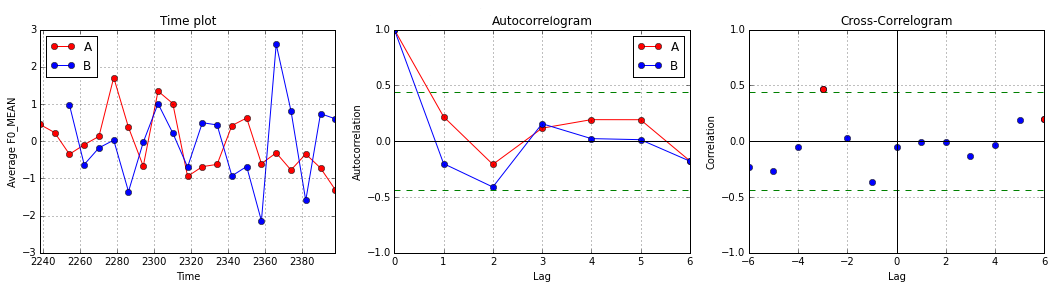
\includegraphics[width=\textwidth]{images/time_plot_with_cross_correlation.png}
\caption{Time-plot producido por TAMA, junto a su autocorrelación y correlación cruzada}
\end{figure}

\newcommand{\squarederr}[1]{
    \sum\limits_{t=1}^n \varnorm{#1}^2
}

\newcommand{\crosscorr}[2]{
  \frac{\sum\limits_{t=|k|+1}^n \varnorm{#1} (#2_{t-k} - \mu_{#2})}{
    \sqrt{\squarederr{#1} \squarederr{#2}}
  } \\
}

\newcommand{\corrdenom}{\sqrt{\squarederr{A}\squarederr{B}}}

En \cite{KOU2008.2} se continúa el trabajo en series de tiempo, y se efectúan análisis tanto para cada serie por separado como para las dos en conjunto, lo cual se llama ``análisis bivariado'' en la terminología de series de tiempo. En este análisis pretendemos analizar ambas series como parte de un sistema y ver cómo se influyen y retroalimentan mutuamente.

Una posible medida del \entrainment se podría obtener midiendo cuánto influye una serie sobre otra, considerándolas a ambas como parte de un sistema donde ambas interactúan. Este \entrainment, entonces, sería direccional: queremos medir cuánto influye el interlocutor $A$ sobre el interlocutor $B$ y viceversa. Puede darse el caso en que ambos tengan fuerte interacción, en tal caso hablamos de \emph{feedback}.

Para medir cuánto se mimetizan las dos series, utilizaremos la función de correlación cruzada (f.c.c) \cite{CHATFIELD}, que mide cuánto se parecen la serie $X$ e $Y$ aplicando un desplazamiento $k$, lo cual nos arroja como resultado un valor entre $-1$ y $1$ (similar al coeficiente de correlación de la estadística clásica). Podemos aproximar la c.c.f. mediante la fórmula de la correlación cruzada muestral.

\begin{equation}
  \label{cross_correlation_definition}
  r_{AB}(k) =
  \left\{
    \begin{array}{ll}
      \frac{\sum\limits_{t=k+1}^n \varnorm{A} (B_{t-k} - \mu_{B})}{\corrdenom} \\ & \mbox{si } k \geq 0 \\
      \frac{\sum\limits_{t=-k+1}^n \varnorm{B} (A_{t+k} - \mu_{A})}{\corrdenom} \\  & \mbox{si } k < 0
    \end{array}
  \right.
\end{equation}

Podemos ver que, si $k \geq 0$, lo que hacemos es, a grandes rasgos, calcular la correlación de Pearson entre $A$ y $B$, pero tomando los $n-k$ últimos valores de $A$ y los $n-k$ primeros de $B$. Si $k < 0$, lo hacemos entre $A$ y $B$, pero desplazando en sentidos inversos. Viéndolo de otra forma, si $k \geq 0$, estamos midiendo cuánto influye $B$ sobre $A$ contemplando un desplazamiento de $k$ puntos; si $k \leq 0$ medimos la influencia de $A$ sobre $B$ a misma distancia. La utilización de estos desplazamientos está explicada en \cite{gravano2015backward}, donde se menciona que la influencia de los hablantes no es necesariamente inmediata sino que puede tener algunos segundos de demora para tomar lugar.


Para cada conversación, se estima entonces el correlograma cruzado, considerando desplazamientos tanto positivos como negativos. Hecho esto, en \cite{KOU2008.2} sólo analizan la significancia de los resultados de la correlación cruzada, enumerando aquellos lags en los cuales esto ocurrió. En la sección \ref{sec:method_entrainment} comentaremos cómo utilizamos la técnica descripta para la medición del entrainment direccional.

